\documentclass[11pt, oneside]{article}   	% use "amsart" instead of "article" for AMSLaTeX format
\usepackage{geometry}                		% See geometry.pdf to learn the layout options. There are lots.
\usepackage[parfill]{parskip}    			% Activate to begin paragraphs with an empty line rather than an indent
\usepackage{graphicx}						% Use pdf, png, jpg, or eps§ with pdflatex; use eps in DVI mode
											% TeX will automatically convert eps --> pdf in pdflatex
\usepackage{amssymb}
%\usepackage{svg}
%\svgpath{{../imgs/}}
\usepackage{comment}						% for \begin{comment}
\usepackage{pifont}							% for \ding
\usepackage{url}							% for "plainurl" support in \bibliographystyle 
\usepackage{hyperref} 						% for \hyperfootnote

% Make clickable footnote
\newcommand{\hyperfootnote}[1][]{\def\ArgI{{#1}}\hyperfootnoteRelay}
	% relay to new command to make extra optional command possible
\newcommand\hyperfootnoteRelay[2][]{\href{#1#2}{\ArgI}\footnote{\href{#1#2}{#2}}}
	% the first optional argument is now in \ArgI, the second is in #1
% Takes at most 3 parameters (see http://www.tex.ac.uk/FAQ-twooptarg.html for info on multiple optional parameters)
% If first parameter isn't given, it's value is '' (empty string in text before footnote reference)
% If second parameter isn't given, it's value is '' (string before visible URL, e.g. 'http://')
% Makes a clickable footnote (alternatively: \url{}) with optional reference in the text as well
% Use 1: \hyperfootnote{www.mywebsite.com}: creates a footnote consisting of a clickable URL
% Use 2: \hyperfootnote[My website]{www.mywebsite.com}: creates a clickable piece of text in the text ('My website') plus a footnote consisting of a clickable URL
% Note: requires the hyperref package.
% Note: use xspace package to add/absorb spaces when necessary (e.g. to avoid a space between the footnote number and a punctuation mark)
% Info on how to define a LaTeX command: https://www.sharelatex.com/learn/Commands

\geometry{letterpaper}                   	% ... or a4paper or a5paper or ... 
%\usepackage{draftwatermark}
%\SetWatermarkLightness{0.9}
%\SetWatermarkText{DRAFT}					% you can use \today
%\SetWatermarkScale{4}

\title{Identity Agents}
\author{Paul Trevithick, The Mee Foundation}
\date{March 3, 2023. Revised \today}							
\begin{document}
\maketitle
\begin{abstract}
Today's app-centric architecture for personal information has helped fuel the rapid growth of internet apps and sites. Unfortunately and concurrently it has reduced autonomy, agency, and privacy for individuals. People lack the technical means to manage the information involved in interactions they have with hundreds of apps/sites and data privacy law has proven inadequate to prevent the disclosure of this data by these apps/sites to other actors. To address these issues we present design considerations for, and the architecture of, \emph{identity agents}.
\end{abstract}

%keywords: personal data, digital wallet, personal datastore, personal data service, personal agent, digital identity, privacy

\section{The status quo} % SECTION 

\subsection{Power}

Sadly, the following quote applies all too well to the internet of today:

\begin{quote}
	``The stronger becomes master of the weaker, in so far as the latter cannot assert its degree of independence --here there is no mercy, no forbearance, even less a respect for `laws'.''\cite{Nietzsche1901}
\end{quote}

The two main levers of power society are technology and law. The technology of the internet has resulted in an imbalance between the power concentrated in the hands of a few and the power, or lack thereof, of individuals. Data privacy law, on the other hand, while often based on sound principles has proven insufficient to shift meaningful power and privacy to individuals.

\subsubsection{Technology}
First we start with a definition to simplify our discussion. We refer to the mobile or local apps, websites, web services, and even other people's digital agents, that a user interacts with as \emph{apps}. 

These apps process personal data in a few different ways: (i) data related to user interactions is stored in \emph{accounts}, (ii) third-party adtech systems track the user and display ads on these apps, and (iii) transaction systems process the user's payment data. We discuss each of these in turn.

\textbf{Account data}. As a user interacts with an app, whatever they type, click, enter, upload is stored in the user's ``account.'' Additional observations, e.g. the kinds of things they click on, and spend time on, are also collected. 

Users have limited power (i.e. control) over their own account data. At best there may be a means to review and update it via an online form. In some cases the app allows the user to download a copy of their account data, although doing so is time-consuming, labor-intensive, and produces dozens of files that the user probably don't know how to use. In some jurisdictions the user has the right to rectify and/or erase account data. Unfortunately, in practice these rights remain almost entirely formal and theoretical due to the unmanageable burden placed on the user to exercise them. 

The app provider may sell the user's account data to \hyperfootnote[data brokers][https://]{theconversation.com/its-time-for-third-party-data-brokers-to-emerge-from-the-shadows-94298} who buy data from a variety of sources, collate information about individuals or groups of individuals, and then resell it.

\textbf{Tracking data}. Tracking is a form of surveillance of individuals by businesses. Businesses gain ad revenue by implementing surveillance using in-app technologies apps (e.g. third-party cookies, transparent pixels, fingerprinting, etc.) that integrate with hundreds of systems managed by the adtech ecosystem.

Tracking data is behavioral data used to infer traits about the individual (e.g. age-range, income level, and many of other demographic and psychographic traits). Advertisers pay to get their messages (ads, images, videos, text, etc.) in front of cohorts with shared traits (called ``audiences'') irrespective of which app a member of that cohort is using. Apps sell ad inventory (i.e. ad ``slots'') to these advertisers. Although some are sold directly, most are sold via ad networks and ad exchanges that take part in a high volume, high-speed real-time auction process called \hyperfootnote[real-time bidding][https://]{en.wikipedia.org/wiki/Real-time\_bidding}. A complex ecosystem of thousands of adtech firms is involved in the supply chain stretching from advertisers, through ad exchanges, to the apps acting in the role of publishers. 

\textbf{Payment data}. Apps that sell products or services leverage payment gateways that allow the app provider to receive funds from the user (e.g. via a payment card). In most cases this involves sending financial data (including identifiers) about the user through financial systems run by banks, credit card associations, and their service providers.

In addition to the privacy risks associated with the flow of payment transactions, some app providers also earn money by selling purchase information to data brokers.

\textbf{Harms}. In the data flows just mentioned, the user is relatively powerless over their data. We live today in what Alicia Solow-Niederman calls an ``inference economy''\cite{Solow-Niederman2022} wherein big data and machine learning are used to infer traits that form new kinds of personal information--often more sensitive than the underlying source data. Harm and risk can rarely be evaluated outside a specific situation\cite{Solove2023}, yet it is useful to list representative types of harm. Individuals:

\begin{itemize}
	\item Are vulnerable to data breaches by any of these thousands of apps.
	\item Have no visibility into what's being gathered, where it's being shared and how it's used.
	\item Can be spammed by marketers.
	\item Are vulnerable to identity theft.
	\item Can be exposed to price discrimination.
	\item Can be exposed to from hiring discrimination.
	\item Can be stalked.
\end{itemize}

\subsubsection{Privacy}

``Debates over privacy are really debates about how power will be allocated in an information society and how much power the humans in that society will get as consumers or citizens.''\cite{Richards2021} Today, despite significant new regulation, the basic approach to protecting privacy hasn't changed since the 1970s. It is often called \emph{notice and consent}. Solove described it using the term \emph{privacy-self management}, as follows:

\begin{quote}
	[T]he law provides people with a set of rights to enable them to make decisions about how to manage their data. These rights consist primarily of rights to notice, access, and consent regarding the collection, use, and disclosure of personal data. The goal of this bundle of rights is to provide people with control over their  personal data, and through this  control people can decide for themselves how to weigh the costs and benefits of the collection, use, or disclosure of their information.\cite{Solove2012}
\end{quote} 

Although well-intended, and necessary, \emph{notice and consent} does not provide people with meaningful control over their data. 

The U.S. population consistently misunderstands the meaning of the term privacy policy.\footnote{``Privacy policies have been widely adopted and are now commonplace. This kind of transparency is good in theory, but less so in practice since it places the onus of privacy on end users. In general, attempts to improve privacy by helping end users have not worked, since most people don't have the time, expertise, or desire to deal with all the nuances of privacy.''\cite{Hong2023}} A majority of Americans believe incorrectly the mere presence of a privacy policy indicates a website will not share information without permission.\cite{Draper2019} 

The problem is well summarized as follows:
\begin{quote}
	When presented with click-through consent, privacy policies or terms of use statements, most people reflexively select ``I agree''. An extensive body of academic research specifically on privacy and data collection notices demonstrates that members of the public don't read them and might not understand them if they did and that many misinterpret their purpose, assuming that the existence of a privacy policy displayed by way of notice means that the entity collecting the data offers a level of data protection when, in fact, privacy notices do not guarantee privacy. Since the terms offered are typically ``take it or leave it'', to decline often results in being denied the product or service one seeks, creating a disincentive for consumers to do anything other than accept the terms.\cite{Flanagan2020}
\end{quote}

``We agree to all these 'privacy notices' so we must have privacy, right? Notice and choice is thus an elaborate trap, and we're all caught in it.''\cite{Richards2021}

\textbf{Progress: GDPR and CPRA}

The most substantive lever for progress has been legislation such as GDPR and CPRA, along with regulatory fines by organizations like the FTC. 

In a growing number of jurisdictions, including Europe under \hyperfootnote[GDPR][https://]{gdpr-info.eu/} and California under \hyperfootnote[CPRA][https://]{thecpra.org/}, the person's \emph{data rights}, (e.g. the right to access, rectify and erase their data), are clearly described. Unfortunately in practice the time and effort required to exercise these rights at each app individually is enormous. The individual must, for example, send written requests to get copies of their data, update it, or have it be deleted. Until these processes are automated by personal agents, in practice these rights don't exist.

\textbf{Privacy and protection of children}

Society agrees to supervise the places children inhabit, protect them from environments they should not encounter, and regulate the products they use. As a result, businesses are not permitted to sell tobacco, alcohol, pornography, handguns, certain kinds of fireworks, and other products and services to minors. However, none of this is true online. In the virtual world children are largely unprotected despite being exposed to wide range of potential harms. 

Many approaches have been proposed and tried without much success. Existing laws have proven to be insufficient, and industry self-regulation has largely failed. Today there is a renewed global push to protect children's safety through stronger laws and regulations. Although some use other approaches\footnote{Such as requiring online services that are likely to be used by young people to default to the highest privacy setting possible for minors, as mandated by California's Age-Appropriate Design Code Act.}, many mandate age verification.\cite{Griswold2023}\cite{Jackson2023} However, privacy advocates and others have shown that many of the mechanisms for verifying age online weaken anonymity and privacy.\cite{Roth2023}

\subsection{Autonomy}

\textbf{Definition}: \emph{freedom from external control or influence; independence.}\hyperfootnote[][https://]{languages.oup.com/google-dictionary-en/}

\subsubsection{Independence} 

We each have a self that embodies our unique individuality. We ``bring'' that independent selfness to our interactions with others. However, online ``we have no \emph{digital embodiment}.''\footnote{Phil Windley, personal communication, September 2022} Our identifiers and their associated account data are provided to us by online service providers (e.g. in the form of a Facebook or an Amazon account) and without them, we don't exist. We can't ``bring'' them anywhere. Anyone who has been banned from a platform, or uses a platform that has been shut down, is sharply reminded that their account and its data exists at the pleasure of that platform. 

Note: Since our discussion applies equally to an online service provider's mobile app, web app, or website, we will simply use the term \emph{app} to refer to all of them.

\subsubsection{Possession} 

In theory, and as we have just discussed, ownership doesn't require possession. That is, with sufficiently strong legal mechanisms (some of which we will propose later in this paper) a sense of ownership can be provided irrespective of where our data is stored and by whom. 

In practice possession tends to shift power to the possessor. Unfortunately, with few exceptions our personal information is stored and managed by service providers. This pattern of what could be called \emph{app-held data} by the \emph{first-parties} we interact with is so common that it's hard to imagine an alternative. Beyond first-parties, our data is also collected and held by \emph(third-parties) (e.g. data brokers) with whom we have no direct interaction. In short, as Johannes Ernst has put it, \hyperfootnote[“everybody has our data … except us.”][https://]{reb00ted.org/personaldata/20210620-who-has-my-personal-data/}. Giving people possession of their data doesn't mean that it doesn't also exist in many other places, but what it does mean is that \emph{at least} we too have it!

\subsubsection{Peer-to-peer}

We lack the ability to directly communicate person-to-person (e.g. chat) with others without having to rely all parties having accounts on the same server. With a few exceptions\hyperfootnote[][https://]{berty.tech}, we don't have the ability to do so \emph{peer-to-peer}--i.e. from one person's device to the other person's device. Instead, we're dependent on servers hosted by intermediaries. Further, whereas it is now standard practice that the content of messages is end-to-end encrypted, the metadata about them (e.g. who a person communicates with, from where, at what time, how often and from which device, etc.) is in many cases visible to the intermediary server.  

\subsection{Agency}

\textbf{Definition}: \emph{the capacity, condition, or state of acting or of exerting power}\hyperfootnote[][https://]{www.merriam-webster.com/dictionary/agency}

\subsubsection{Access}

Privacy laws such as the GDPR provide the individual the following rights over their personal information regardless of where it is stored:
\begin{itemize}
	\item Right to rectify
	\item Right to access
	\item Right to erasure
\end{itemize}

These laws are largely not actionable. Without APIs on the service provider's side, as well as personal software to consume them on the individual's side, the burden required to exercise these access rights is unbearable.

\subsubsection{Portability}

Our account identifiers and associated human data are bound to specific online service providers and can't be moved freely from one to another. In other words they are not \emph{portable}.

In many jurisdictions service providers are required by law to provide individuals with access to their data, but they usually offer this by means of a set of files emailed to the individual as an attachment several hours or days after the request. There are significant problems with implementing portability in this manner. First, it is tedious, manual and slow. Service providers don't support data ``export'' APIs, so an individual can't use technology to automate the process. Second, the individual ends up with dozens of sets of files (one set from each provider) that are not largely unintelligible to them. 

Beyond access and export problems, providers generally don't provide ``import'' APIs to allow the individual to upload their data. Even if an individual could import their data, it first must be transformed into the format of the recipient, since each provider uses their own format. The result is a lack of practical portability.

Advocacy groups, including the EFF, are pushing for interoperability as an antidote to corporate concentration. This is good, but they should insist that apps implement import/export APIs that can be leveraged by agents such as identity agents. ``A new regime of interoperability can revitalize competition in the space, encourage innovation, and give users more agency over their data...''\cite{Cyphers2021} 

\section{Related Work} % SECTION 

Many initiatives have arisen to address the challenges we've described. We mention a few of them here.

The lock-in and lack of data portability and interoperability between service providers is being fought using both policy and technical means\cite{Doctorow2021}\cite{Cyphers2021}. 

Work related to re-decentralizing the internet includes: \hyperfootnote[rececentralize.org][https://]{redecentralize.org}, \hyperfootnote[DWeb principles][https://]{getdweb.net/principles/}, \hyperfootnote[The Web3 Foundation][https://]{web3.foundation/}, \hyperfootnote[the Decentralized Identity Foundation(DIF)][https://]{identity.foundation}, \hyperfootnote[``local-first" software principles][https://]{inkandswitch.com/local-first/}, \hyperfootnote[ProjectVRM][https://]{projectvrm.org/}, \hyperfootnote[Blue Sky][https://]{blueskyweb.xyz/}, and Berners-Lee's \hyperfootnote[Decentralized Information Group][https://]{dig.csail.mit.edu}. 

See also work on \emph{personal agents} \footnote{What Mozilla calls a \hyperfootnote[\emph{user agent}][https://]{developer.mozilla.org/en-US/docs/Glossary/User\_agent}}--software tools that work (i.e. provide agency and power) ``on the individual's side"\footnote{Project VRM\cite{Searls2019} refers to this as ``tools for individuals to manage relationships with organizations'' to which we would add ``...or with other individuals."} for, and \emph{exclusively} on behalf of, the person. Personal datastores and the \emph{self-sovereign identity}\cite{Preukschat2021} movement are squarely aimed at addressing our lack of autonomy.

Particularly relevant is work on personal datastores\footnote{Examples of open-source personal datastores include \url{https://solidproject.org} Decentralized Web Nodes(DWN)is relevant here. For more about personal datastores see \url{https://wikipedia.org/wiki/Personal\_data\_service}}. 

Also relevant is work on ``local-first" software.\cite{Kleppmann2019}

\section{Design Considerations} % SECTION 

In this section, we discuss design considerations for solutions that intend to address the symptoms described in the previous section. We first discuss design considerations related to ensure that agents enforce the user's privacy data rights and are trustworthy. Then, we turn to functional requirements necessary for an agent work with legacy apps as well as new/adapted apps that work within a new trust framework.

\subsection{Data rights}

In a growing number of jurisdictions new privacy regulations promise \emph{data rights} to access, correct and delete the personal information about users that is managed by apps providers. In practice the burden of exercising them across hundreds of apps is unmanageable. Automation on the user's side is required. Agents can provide this automation, although this is only half of the answer. The other half involves constraining how apps use this user's data, and having them implement APIs that the agents can use--this is described below in the section on Trust Frameworks.

\subsection{Convenience}

Convenience is one of the most important design considerations to drive user adoption of agents. An agent must automate the work of controlling and managing a person's own information. 

\subsection{Inclusivity}

Agents must be affordable by all socio-economic classes--not just those better off. For this reason, solutions that incur monthly hosting cost are disqualified. For virtual (web-based) agents this creates a significant funding challenge. The situation is better for \emph{local} agents that run on the user's device, although there may be additional costs incurred for any additional storage required for larger on-device datastores.


\subsection{Loyalty to the user}
Much of the power asymmetry described in the first section is created by the economic incentives for online service providers to monetize user's personal information. They do just enough in the user's interest ensure that they keep using the service and co-creating personal data to monetize. Personal data, after all, is now considered to be an asset class--the more of it that's collected the better. For a user to trust that their agent works \emph{exclusively} on their behalf, the \emph{agent provider} (i.e. organization that develops and provides it) must not have an economic incentive to be disloyal to the user. This can be ensured by designing agents so that the personal information that they process is never accessible to the agent provider. This largely eliminates the need to trust the agent provider organization, their security infrastructure, their processes, etc.

\subsection{Open source agents}

The transparency of open-source software can build confidence that any agent built from this source code is trustworthy. In open-source software the source code is visible to anyone to review and audit to ensure that the agent is secure, free from vulnerabilities, works in the person's interest, and performs as expected.

\subsection{Trustworthy agents}

Users need to trust that the agent developer/provider organization is itself trustworthy. Their financial incentives should be aligned with the user's interests. Nonprofit or similar organization structures can increase trust that agents offered by this organization have no financial incentive to exploit the user's data for its own advantage. 

\subsection{Trust Framework}

Once data is shared from an agent to a first-party app there are no technical means to constrain what the recipient can do with it. No technical means, for example, can prevent them from selling it others. Instead, legal means (trust frameworks) must be employed. 

Some apps will be willing to join a trust framework and \emph{license} the user's information received from the user's agent. If so, they would agree to the terms of a license agreement which include terms which respect the person's privacy rights. This contract is signed by a trusted organization\footnote{These kinds of organizations have been variously described in the literature as ``data unions,'' ``data coalitions,'' ``Mediators of Individual Data'' (MIDs) by Lanier et al.\cite{Lanier2018}, etc.} that represents the community of identity agent users thereby making the processes effortless for them. Lastly, this organization is responsible for enforcement of the contract's terms, again, on behalf of the user.
\begin{comment}
	mention trust framework?
\end{comment}

\subsection{Human-centricity}

Many of the challenges described in Section 1, The status quo, have their origin in an architecture that is \emph{provider-centric} rather than \emph{human-centric}. The internet includes millions of providers, each offering their own app[s]. In this provider-centric model each provider's app sees a narrow slice of the individual through the lens of their direct interactions with them. 

For the individual the situation is reversed. They sit at the center of a hub with many dozens of connections to apps radiating outwards from them. Even for a single app there is considerable burden for the person to enter and update personal information, payment details, and preferences, and review privacy policies, and set cookie preferences, and so on. Multiplied by perhaps one hundred connections, the resulting burden is unbearable. 

Tools to manage these chores must sit on the person's side, and work on their behalf across all of them. Technologies of this kind, that empower a person across multiple apps, e.g. browsers and password managers, are called are \emph{user-agents} since they act as agents of the person. 

\subsection{Metacontextuality}

Zuckerberg once said that ``[h]aving two identities for yourself is an example of a lack of integrity"\cite{Kirkpatrick2011}. However, even if one could force everyone using a single platform (e.g. Facebook) to have a single identity\footnote{Note: \emph{identity} is term we prefer to avoid due to its semantic ambiguity, but this is the word he used.}, this approach is clearly unworkable for a solution that represents the person across multiple, widely varying systems and contexts. People need the freedom to be themselves--selves that are complicated and messy. Our identities vary depending on whom we are interacting. We choose to express different parts of ourselves within different contexts. Not only are the attributes we share different, but the values of one attribute may be different in different contexts. 

\begin{quote} 
	``[A]t various times in the same day, virtually every adult can be a friend, a worker, a supervisor, a citizen, a mentor, a student, a musician, a customer, a lover, a child and a parent. Each of these roles demands different behavior and different aspects of our selves, aspects that need not be consistent. We behave, for example, in different ways with loved ones than with those we encounter in commercial or professional settings. Even among our loved ones, we behave very differently (and often show very different sides of ourselves) to our children, our parents, and our sexual partners. But this is not dishonest, nor is it inconsistent. At the very least, it's no more inconsistent than is the complicated nature of having a self. It is human.''\cite[p122]{Richards2021}
\end{quote}

Let's look at a person's age as an example. We see that across contexts they might share, their exact chronological age among their close friends, a fictional age to a music recommendation service, no age at all in contexts wherein doing so might cause discrimination against them, or a merely a statement that they exceed the legal drinking age. 

In his \hyperfootnote[last public speech][https://]{www.youtube.com/watch?v=9DExNTY3QAk}  
\hyperfootnote[Kim Cameron][https://]{en.wikipedia.org/wiki/Kim\_Cameron\_(computer\_scientist)} introduced two useful definitions based on archaic English:

\begin{itemize}
\item \textbf{Selfness}: The sameness of a person or thing at all times or in all circumstances. The condition of being a single individual. The fact that a person or thing is itself and not something else. Individuality, personality. 
\item \textbf{Whoness}: A distinct impression of a single person or thing presented to or perceived by others. A set of characteristics or a description that distinguishes a person or thing from others. 
\end{itemize}

Figure~\ref{fig:multiple-contexts} illustrates these concepts and introduces the notion of context.

\begin{figure}[htbp]
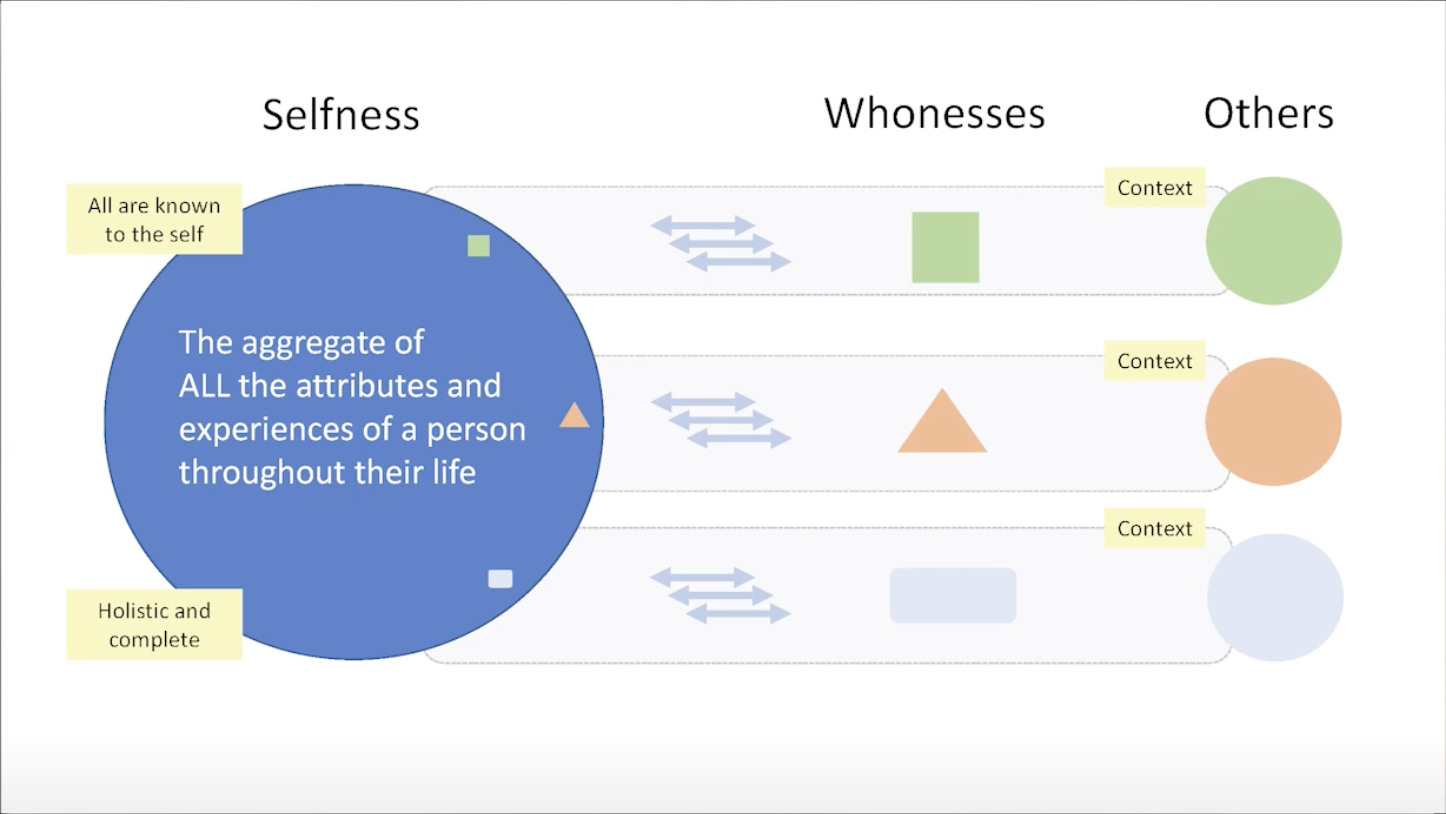
\includegraphics[width=\textwidth]{./images/selfness-and-whoness-larger.png}
\caption{Multiple whoness-contexts around a single selfness}
\label{fig:multiple-contexts}
\end{figure}

Using these terms we can say that in everyday life people have one \emph{selfness}, but they have many, context-dependent \emph{whonesses}. Any solution must be meta-contextual--it must embrace and support the complicated, multi-contextual nature of our lives.

\subsection{Local-first}

In this section we argue that a local-first architecture is preferred. 

A user's personal datastore may be on-device or in the cloud. By \emph{on-device} we mean that the individual's datastore and processing is on their own phones, laptops, and/or home servers. By \emph{cloud-based} we mean that the person's datastore and processing lives in the cloud (e.g. on a \hyperfootnote[SOLID][https://]{solidproject.org} pod). The \hyperfootnote[local-first software][https://]{www.inkandswitch.com/local-first/} principles are highly relevant. Although there are other points of view, we contend that if many people are using the solution, having a personal datastore on-device is more secure than in the cloud. Even if each alternative were equivalently secure for a single person, a cloud-based architecture by nature aggregates large numbers of personal datastores at one cloud service provider location, and thereby creates a much larger economic incentive for hackers. 

\subsubsection{Synchronization}

A user may have two or more identity agents running on multiple devices each of which is only intermittently connected to the internet. The user's data needs to be kept consistent across these identity agents and devices, at least eventually. This requires that the person's identity agents implement data replication and syncing between themselves in a peer-to-peer (P2P) fashion. Unfortunately pure P2P communication between identity agents running on differing device platforms remains an unsolved problem and intermediate relay servers are sometimes required. 

Since relays are a necessary part of the deployment architecture, for privacy, autonomy, trust, and security reasons they are subject to their own design considerations. We touch on a few of them here. For the very few people who are able and willing to self-host their own relays, the relay needs to be free, open-source and easy to build and deploy. Everyone else will have to trust some external administrative authority. Hopefully relays will be available freely or at very low cost. In either the self-hosted or external case, the relay needs to be trusted. For this reason its source code should be open, and the relay should only store encrypted data. It should store message data only while waiting for the recipient agent to come online.

\subsubsection{Backup} 

One disadvantage of \emph{noncustodial}, on-device architectures (as compared to cloud-based architectures) is the vulnerability agent users who are not diligent about backing up their devices (e.g. to an online service) face of losing their agent-managed personal data. For people with more than one device this is less likely since data is replicated (as mentioned above) across their devices, and a repaired or replaced device's data can be restored from one of the person's other devices. There remains of course the worst-case scenario wherein the person hasn't backed up any of their devices and all of them are lost or damaged simultaneously. 

Identity agents could implement backup/restore approaches that would provide recovery from even this disaster, however they are themselves complex and problematic. The agent's data must be stored in remote storage location(s) and encrypted using a master passphrase that the person must never be able to forget or lose. To do this, various approaches including sharding, \hyperfootnote[shared secrets][https://]{en.wikipedia.org/wiki/Shamir\%27s\_secret\_sharing}, and social recovery have been proposed, although this remains an area of active research. 

\subsection{Delegation}

In \emph{A Human Rights Approach to Personal Information Technology}\cite{Gropper2022} Gropper asserts that there is an architectural principle that must be adhered to in order to respect human rights [e.g. to privacy]. He identifies three universal components:

\begin{itemize}
\item \textbf{Authentication} (signing-in and signing documents)
\item \textbf{Request} for information (e.g. forms, searches, conversations)
\item \textbf{Storage} (e.g. labs, prescriptions, social contracts, transactions [, other human information])
\end{itemize}

He then asserts what could be called the \emph{Gropper Principle} as follows (our words, his ideas):
\begin{quote}
``Any system that respects the human right to privacy must not bundle authentication, request, and storage.''
\end{quote}

In his presentation\hyperfootnote[][https://]{identiverse.com/idv2022/session/841489/} at the 2022 Identiverse conference provides additional detail (see \hyperfootnote[slides][https://]{drive.google.com/file/d/1lwaMVkG4kLi7z6cXhqMx-DGkUww9azW3/view}). It explains that only a decentralized architecture can implement the Gropper Principle because each of the three components needs to be implemented separately. For this to work in an open world with multiple alternative component providers, there will need to be a convergence on open standards between these three components. 

\section{Identity Agents} % SECTION 

 \emph{Identity agents} are a solution to the problems described in the first section that takes into account the design considerations in the second section. An identity agent, gives individuals control over their personal information as they interact with websites, mobile apps, and other people's identity agents through a combination of technical and legal mechanisms. It combines a legal contract and a trusted, personal agent\footnote{Similar ideas have been proposed by others. See \emph{personal user agents}, in \cite[p24]{Flanagan2020}} with a traditional digital agent\cite{Graham2023}. 

We envision two kinds of identity agents, \emph{local} and \emph{virtual}. A local agent is a native app (e.g. written in Swift on iOS, Kotlin on Android, etc.) that runs on a user's devices (e.g., mobile phone, laptop, etc.). It maintains a local, private database of the user's personal information. By default, none of this information is shared with any other entity. When an app wants to know something about the user, the user uses their agent to share as much or as little as they wish. A virtual agent, is a cloud-hosted (or privately hosted) web app that does not include a personal datastore. 

Apps can request personal information from, and provide information to, an identity agent using a wide variety of data sharing protocols. The information may flow between the first-party and the agent in one direction, the other direction or bi-directionally. It may use whatever data formats and schemas are defined by that first-party. The data being exchanged may include structured data, unstructured data, or digitally signed documents (e.g. Verifiable Credentials, etc.). 
\begin{comment}
	Talk about using browser extension as a proxy for first-parties that don't provide real-time API access to personal data 
\end{comment}

The Mee Foundation is developing a Mee Data Network (MDN) specifically designed for first-party to agent communications. It defines a trust framework wherein first-parties \emph{authorized} by The Mee Foundation implement specific APIs and to agree to the terms of a data sharing license. This license requires that they abide by certain privacy principles in how they handle the individual's data (e.g. requiring explicit consent for collection, processing, storage and sharing of the person's data) as well as implement the MDN APIs. These APIs enable \emph{private sharing} between the identity agent and the first-party. Private sharing allows the user to share personal information with confidence that it remains under their control. Following intellectual property law precedents, the user licenses their information to the first-party rather than transferring a copy of it in the hope that the first-party will treat it with care. Using their agent, the user can exercise their rights to access, correct and delete their information stored by the first-party.

\subsection{Benefits for the individual}

\subsubsection{Privacy}

An identity agent increases the user's privacy as follows:
\begin{itemize}
	\item If the identity agent includes a browser extension component, it can add the \hyperfootnote[Global Privacy Control][https://]{globalprivacycontrol.org} field in the HTTP header expressing the user's privacy preference. The extension may also include the ability to delete third-party cookies and other kinds of trackers used in surveillance advertising. Agents can participate in new, \emph{private advertising} networks, that don't rely on cookies, trackers, data brokers, etc. but instead rely on user profiles that are anonymized, and never shared outside the ad network. 
	\item If the agent interacts with apps that are part of the MDN, these apps agree to process the user's personal information under the terms of MDN License. By default, the app can't sell, transfer or share the user's information without their consent. 
\end{itemize}

\subsubsection{Protection of Minors}

Minors can be given a special child-oriented identity agent by their guardians. This kind of agent is an enabler to  provide the minor with an age-appropriate experience online. The guardian would register their minors on a third-party age verification service and issue into the minor's agent an age verification credential. When the minor uses a first-party app, the agent can signal that the minor wishes to have an age appropriate experience. In response the app can request the age verification credential from the minor's agent and adapt its experience accordingly.

\subsubsection{Autonomy}

Identity agents provide individuals with digital embodiment of themselves. Over time, the agent develops rich, context-specific data profiles about them. This embodiment can move autonomously under the user's control between first-party apps. A \emph{local} agent can do so independent of any external administrative authority. 

Identity agents reduce lock-in, because they provide data portability. They provide a convenient way for the individual to retrieve their information from one app, and share it with another. 

As usage of agents grows, surveillance free, end-to-end encrypted communications interconnect these users. These communications can be designed with minimal reliance on cloud-based relay servers which are often needed to buffer messages to endpoints that are temporarily offline.

\subsubsection{Agency}

\textbf{A foundation for Personal AI}

Rather than requiring individuals to trust a shared AI-in-the-cloud service with all of their sensitive personal information, a better approach is to have the \emph{Personal AI} algorithms run on the individual's devices. These algorithms read and write personal information to/from the person's agent.\footnote{Iron Man's \hyperfootnote[J.A.R.V.I.S.][https://]{en.wikipedia.org/wiki/J.A.R.V.I.S.} is an example of this architecture and offered Iron Man complete privacy.}

\textbf{Logging in without passwords}

Identity agents enable the user to log in to apps using a variety of password-less authentication technologies. The agent knows who the user is because the user authenticates to it, so the agent can represent the user in their interactions with apps, and can do so without revealing correlatable identifiers. This is both private and convenient.

\textbf{Wielding credentials}

In real life an individual can, say, present their driver's license to a wine seller to prove that they are of drinking age because the wine seller trusts the license issuer. This interaction is privacy-respecting because the presentation interaction is never disclosed to the issuer. This driver's license use-case involves the individual \emph{wielding} a trust credential. Unfortunately, there is no commonplace way to do this online. There's no standard way to be issued a credential, hold it in a digital agent (acting as a digital wallet), and then present it to another party. With a few, domain-specific exceptions (e.g. cryptocurrency), there is no standard online method for an individual to prove something one party states about them, to another party. Digital wallets are emerging to meet this need and this wallet-like capability is included in an identity agent.

\textbf{Automated data presentation}

Apps rely on form filling and other kinds of tedious, manual data entry because individuals lack the ability to \emph{digitally} present personal information about themselves. Individuals must manually re-enter personal information into each app, endlessly repeating themselves. They lack an agent that can automatically present information on their behalf.\footnote{The credential presentation interaction just mentioned is another example of this.} 

This endless repetition is a symptom of the internet's silo-ed architecture wherein each app maintains its own database of personal information. The individual has the hassle of repeated data entry, and the app offers a less-than-optimal user experience. With an identity agent the user no longer has to repeat themselves as they move from app to app.

This inability to present ourselves digitally is a contributing factor to the concentration of corporate power on the internet. For example, it's simply easier to buy something from Amazon because so many of us have already entered so much information to them. We have a preferential attachment to Amazon that goes beyond their intrinsic advantages. Continuing with the shopping example, agents can represent an individual to any e-commerce website, and thereby provide an same Amazon-like, frictionless user experience that can mitigate corporate concentration and ``natural'' monopolies. 

\textbf{Infer and present ad profiles}

An agent can generate on-device an ad profile by inferring traits from an individual's browsing behavior. The agent's user can review and edit this profile, and may choose to share it with apps that are supported by interest-based \emph{private} advertising technology. This approach eliminates the need for surveillance by third-parties using cookies and other tracking technologies. It is similar in design to \hyperfootnote[Google's Topics API][https://]{developer.chrome.com/en/docs/privacy-sandbox/topics/overview/}.

\textbf{Delegation}

In the offline world one entity can grant access to some resource to another entity. For example, an individual can give their car keys to a friend, so they can borrow their car. At present, there is no standardized way to do this online. This is especially problematic in healthcare scenarios where a healthcare provider needs access to health-related data about a patient, but the patient is not in a situation where they are able to provide it by themselves and must instead rely on someone else, e.g. a family member to grant the needed permission. In the online world each service provider not only possesses the individual's data, but they manage it in such a way that it is impossible for the individual to delegate rights to it to others. 

\textbf{Content filtering}

Social networking platforms have replaced human content editors with algorithmic filters. Individuals may think that they are seeing a balance of content whereas in reality they are trapped in what Pariser called ``filter bubbles."\cite{Pariser2011} Pariser's recommendation is that if platforms are going to be gatekeepers, they need to program a sense of civic responsibility into their algorithms, they need to be transparent about the rules that determine what gets through the filter, and ``they need to give user control of their bubble.''\cite[p66]{McNamee2020} Agents can achieve this.

\textbf{Account management} 

The individual carries the burden of maintaining the timeliness and consistency of their account information at hundreds of apps. For example, updating contact or credit card information at each is tedious, time-consuming and encourages the individual to spend more time at sites that already have their information. The relative convenience of shopping on Amazon vs. other e-commerce sites is partly a consequence of the individual not having an easy way to manage and update their personal information at multiple sites--it's just easier to buy things on Amazon because Amazon already has all of their personal information.

%\subsection{Benefits for businesses} - to be written                                                             

\section{Implementation} % SECTION 

An identity agent sits at the center of an architecture wherein the user's interactions with apps radiate out from it. ``When we put the user at the center, and make them the point of integration, the entire system becomes simpler, more robust, more scalable, and more useful.''\cite{Andrieu2007}

This human-centered architecture necessitates that an agent must be, using the term \emph{protocol} loosely, protocol-agnostic. Consider the user's interactions with four apps. One might want to know the user's email address, it might ask for it in a web form. The agent would use its form-filler ``protocol'' to fill in the value. The second might support password-less sign-in (e.g. using OpenID Connect) that leverages an agent acting as the so-called \emph{identity provider}. The third might request a digital driver's license credential. The agent, acting as a digital wallet, can present this credential--a credential that it had presumably been installed into it from a fourth credential-issuing app. 

\subsection{Self and Contexts}

The identity agent represents both the person's single \emph{selfness} and a set of \emph{whonesses}, each used in the context of their interaction with a different app.

The selfness of the person is represented by a person entity in a data container called the \emph{self}. The person entity in the self is the point of integration across contexts each of which may use differing identifier namespaces, protocols for communication, and data schemas. The contents of the self are holistic and therefore quite sensitive and would normally not be shared with others. 

Each context is represented by a \emph{context} data container. A directed \emph{correlation} link points from an entity in the self to the entities representing the person in each context. To ensure privacy, only the person knows that each of these separate contexts contain representations of them. Each context represents an interaction via some communications protocol with an external app. 

We can illustrate these concepts with a simple example. A person named Alice might play a game on a gaming app using the id DevilSpawn666, communicating on a social networking site as @alicewalker, subscribing to the Olde York Times as alice.walker@gmail.com and shopping on a shopping site also using alice.walker@gmail.com. Figure~\ref{fig:four-contexts} shows a simplified view of how this is represented:

\begin{figure}[htbp]

\includegraphics[width=\textwidth]{./images/example1.png}
\caption{Alice in four contexts}
\label{fig:four-contexts}
\end{figure}

In our example Alice has four digital relationships called \emph{connections}. Each of the four connections shown in the diagram has only a single context, although in general a connection may be represented by more than one context. Since, as will be described more fully later, a context is associated with exactly one communications protocol, in cases where N communications protocols are used in a single connection, the connection will contain N contexts. 

\subsection{Functionality}

Figure~\ref{fig:functionality} summarizes the functionality of an identity agent, and contrasts the local vs. virtual variants. The upper rows list a set of connectors each implementing a different protocol. The lower rows list a set basic identity agent functions. The ``BX'' term is an abbreviation for a browser extension. The ``Agent SDK'' refers to a reusable component that can form the heart of a local identity agent, or can be used as a satellite component embedded in a relying party's app. The cells in light and dark green show the progress of implementation work being led by The Mee Foundation. 

\begin{figure}[htbp]
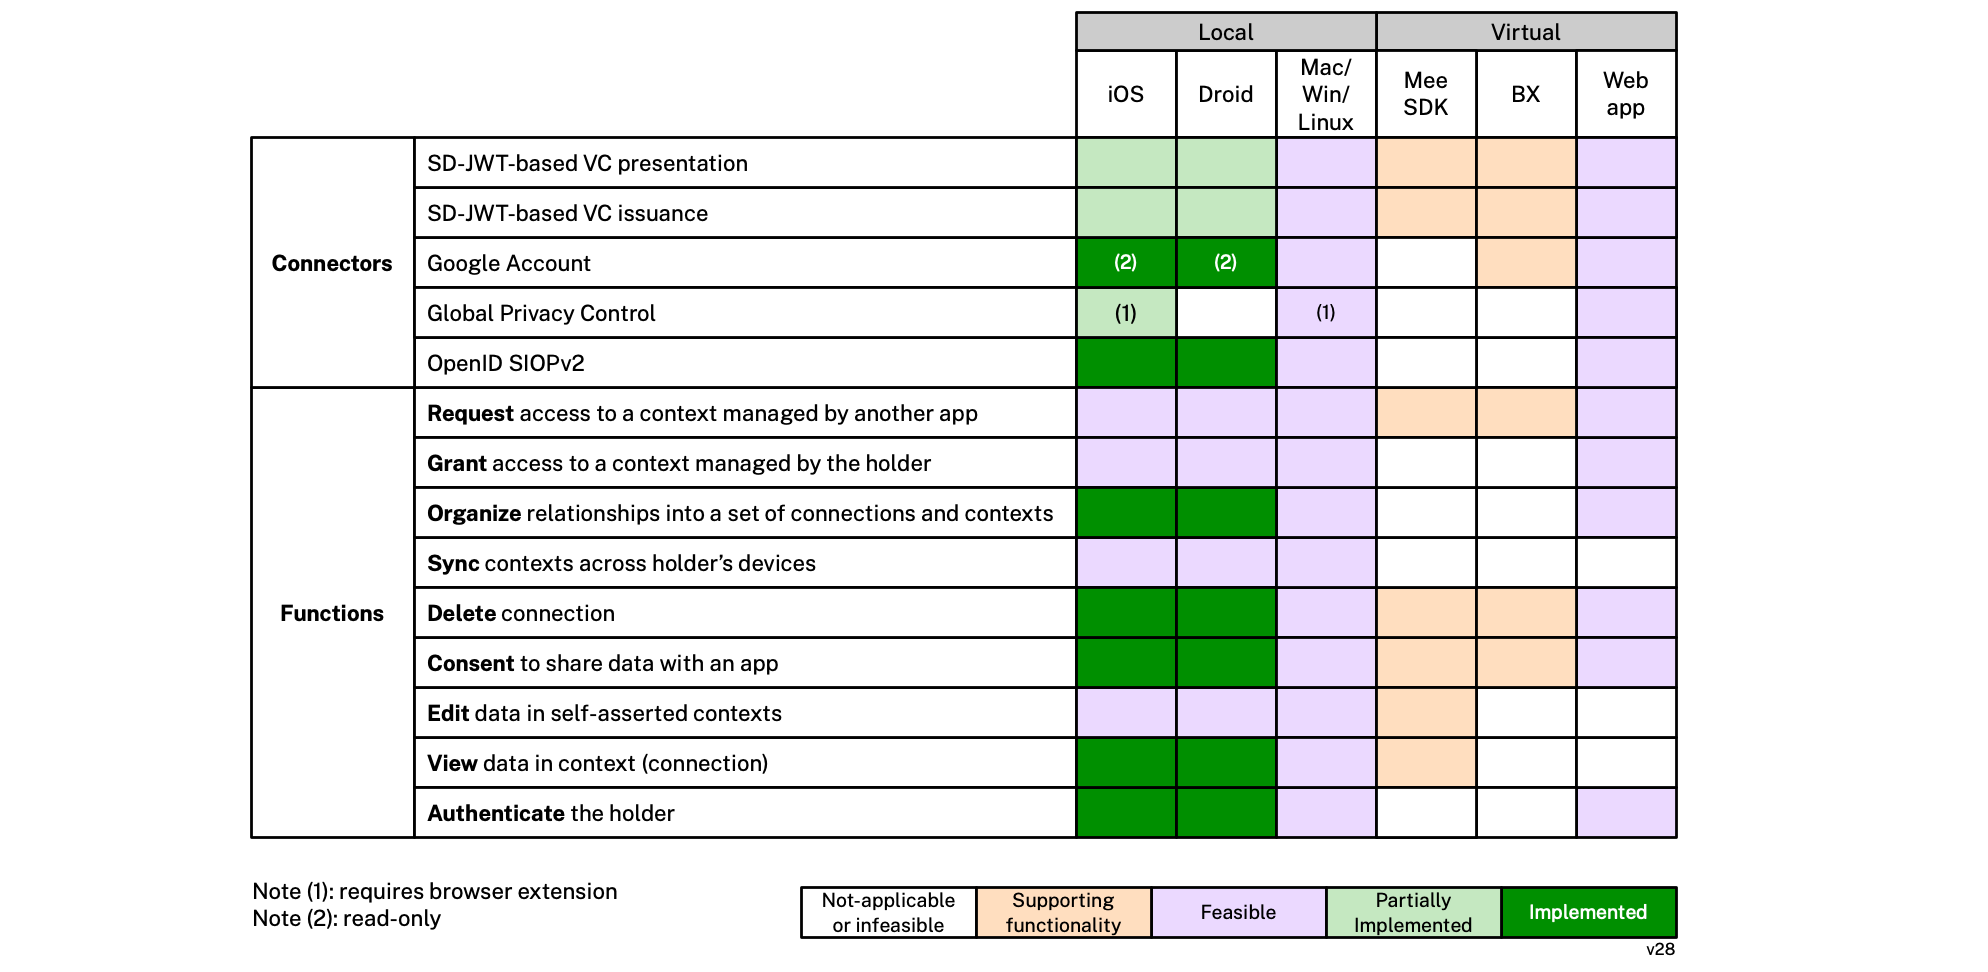
\includegraphics[width=\textwidth]{./images/identity-agent-functionality.png}
\caption{Identity Agent Functionality}
\label{fig:functionality}
\end{figure}

\subsubsection{Connectors}

An identity agent is a tool that allows its user to manage data \emph{connections} with apps (including other people's identity agents). Since a variety of communication protocols and data storage approaches are involved in these connections, identity agents are extensible via \emph{connectors}. 

Here are a few examples of connectors:
\begin{itemize}
\item SD JWT-based VC presentation - present Verifiable Credentials from the identity agent
\item SD JWT-based VC issuance - store a Verifiable Credential in the identity agent
\item Google Account - pull data from myaccount.google.com 
\item Global Privacy Control - sends a ``Do Not Sell My Personal Information'' signal to apps
\item OpenID SIOPv2 - allows the person to authenticate with an app without using passwords, without first creating an account, and with surveillance by an external so-called \emph{identity provider}.
\end{itemize}

\subsubsection{Functionality}

Here are user functions of an agent:

\begin{itemize}
\item \textbf{Organize} the relationships the user has with other apps into a set of connections and contexts.
\item \textbf{Request} access to a context managed by another app.
\item \textbf{Grant} access to a context managed by the user.
\item \textbf{Sync} contexts across user's devices.
\item \textbf{Delete} all data associated with this set of contexts.
\item \textbf{Consent} to share data with an app.
\item \textbf{Edit} data in self-asserted contexts within a connection.
\item \textbf{View} data in a context (connection).
\item \textbf{Authenticate} the identity agent user.
\end{itemize}

\subsection{Architecture}

The multi-layered architecture of an identity agent is shown in the center of Figure~\ref{fig:architecture}. 

Terms such as \emph{self}, \emph{context}, \emph{connection}, and \emph{protocol} used in the following are described in section \ref{data_model_subsection} where we describe the Persona data model.

\begin{figure}[htbp]
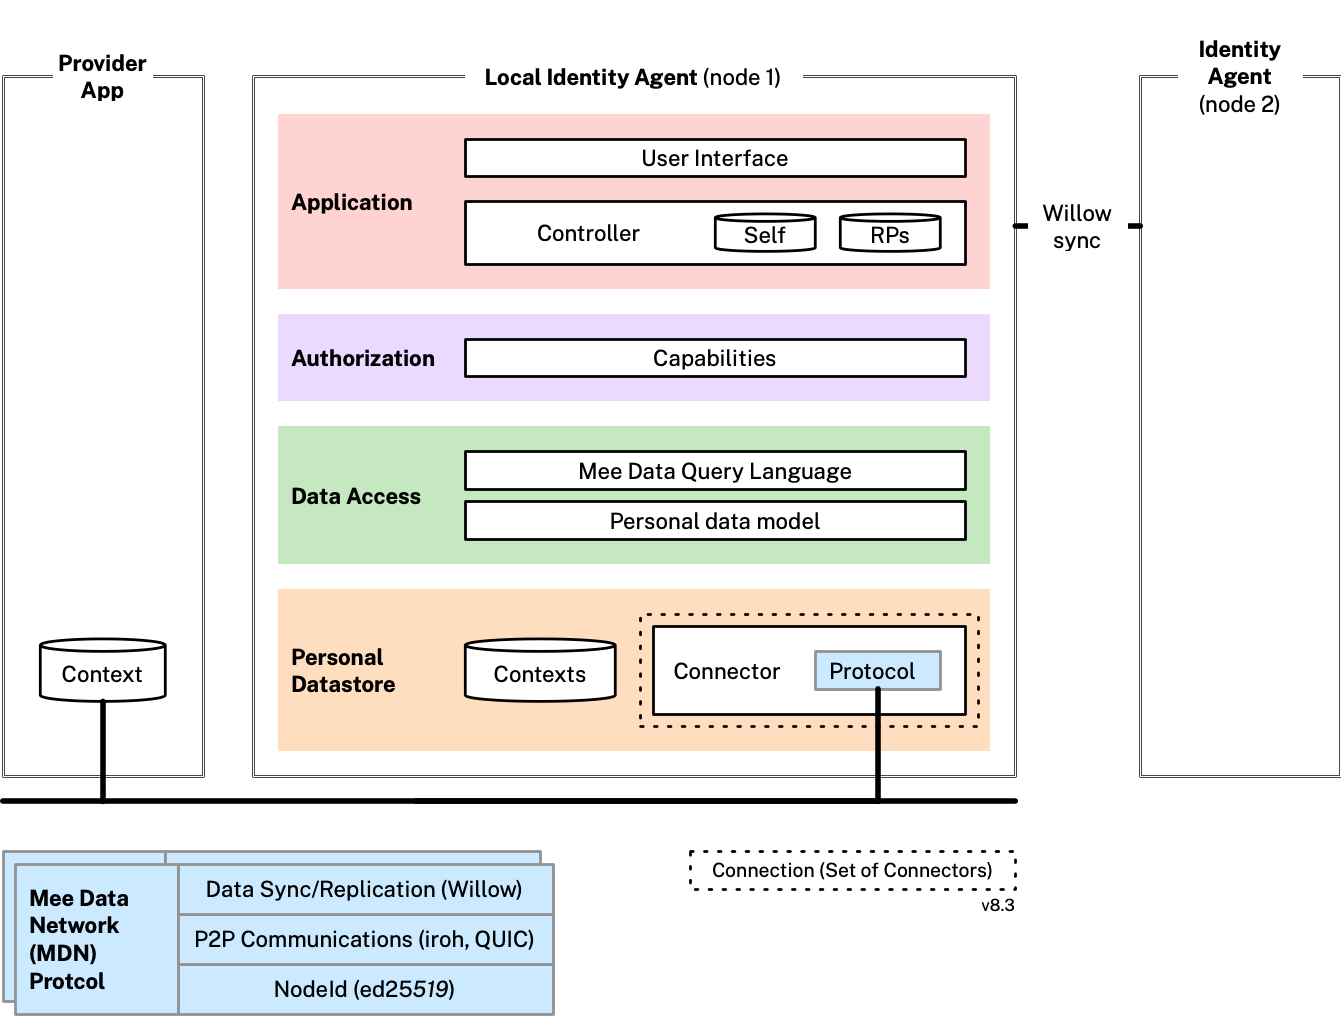
\includegraphics[width=\textwidth]{./images/architecture.png}
\caption{Identity Agent Architecture}
\label{fig:architecture}
\end{figure}

\subsubsection{UI Layer}

User Interface (UI) component provides a user interface to manage the individual's data sharing relationships with apps. Using this UI the user can add and delete connections. Within each connection they can consent to data shared from their agent, see what data is involved in the connection, and in some cases edit attribute values.

\subsubsection{Controller layer}

The controller layer handles requests from the UI. It translates these requests into the Controller component. The Controller manages the Self and the RPs data containers. It updates the attributes of Person objects in contexts via the Data Access component. It is responsible for creating and deleting connections. Lastly, it is responsible for replicating the Self and RPs data containers to other identity agent replicas.

\subsubsection{Authorization Layer}

The Authorization Layer contains the user's \emph{Authorization Server} which responds to requests for access to the individual's contexts--contexts which are managed by the data access layer described below. The AS sends these requests to the controller layer (which may in turn call back to the UI Layer) to allow the user, either interactively or by policy, to grant or deny them. These requests may be from service providers who integrate the identity agent SDK or from individuals' identity agents.

\subsubsection{Data Access Layer}

The Data Access component is responsible for management of the user’s data whether it is stored locally, replicated on another of the user's identity agents, or managed by a service provider. It exposes data contexts via the Controller to the User Interface where it can be viewed and in some cases edited. It is responsible for replicating local contexts to other identity agent replicas.

\subsubsection{Context Storage Layer}

This layer persists local data contexts (some of which may be accessed by Connectors). Data managed by the resource server is encrypted using FIPS-compatible algorithms. Note: this layer is only present in a local, not a virtual, identity agent.

\subsubsection{Connectors}

Now that we've described the horizontal layers of an identity agent, we turn to the \emph{connector} extension point. An identity agent typically has multiple \emph{connections} each of which is implemented by one or more \emph{connectors}. Each connector has a communications aspect and a storage aspect.

\emph{Communications aspect}. A connector implements the communications protocol used by the other party (e.g. a service provider or another person's identity agent). We use the term protocol very loosely since the nature of the other party varies considerably. It could for example be an API of a service provider, another person's identity agent, an authentication protocol exposed by an endpoint, or something entirely different.

\emph{Storage aspect}. A connector persists its state in a context container managed by the Data Access component. The Data Access component requires this context state to be represented in the Persona data model, so the connector is responsible for dynamic, bidirectional schema transformation between the data model of the protocol and the Persona data model.

\subsection{Physical architectures}

A local identity agent includes all logical layers mentioned in the previous section, deployed as a native application on a mobile or laptop device.

A virtual agent is a physically distributed system made up of a web app communicating with multiple ``satellite'' Agent SDKs. The web app implements all but the Context Storage Layer mentioned in the previous section. The \emph{Agent SDKs} we refer here to are shown at the left of Figure~\ref{fig:architecture} and embedded within an RP's app. Figure~\ref{fig:virtual-agent-deployment} shows a single virtual agent and three satellite SDKs. The leftmost Agent SDK is embedded within an RP's web app. To the right of this is a Agent SDK embedded within an RP's local on-device app. On the right a Agent SDK is embedded within a web browser is shown acting as a scraping/filling proxy for yet another RP's web app. 

\begin{figure}[htbp]
	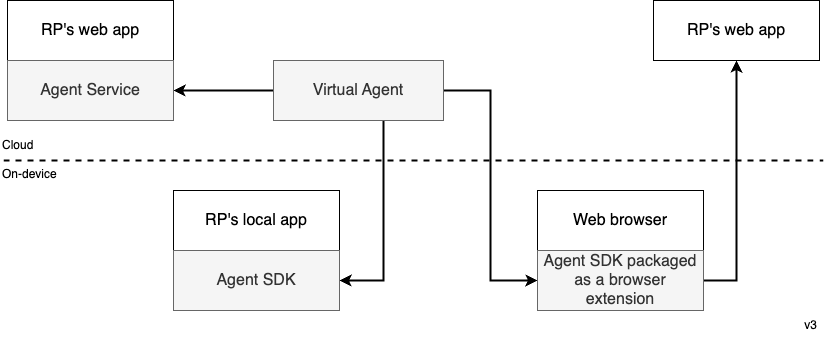
\includegraphics[width=\textwidth]{./images/virtual-web-app.drawio.png}
	\caption{Virtual agent deployment}
	\label{fig:virtual-agent-deployment}
\end{figure}

\subsection{Persona Data model}\label{data_model_subsection} 

This section describes the data model of an agent. The user's data may be replicated across multiple identity agents on different devices, but we focus here on the logical model, not these replicas. The data model can be thought of as a two level hierarchy of data containers each of which holds \emph{Person} instances representing the user. The top layer consists of a single \emph{Self} container. The bottom layer consists of \emph{Context} containers.

These Person instances are connected into a directed graph that spans these  levels of containers. The singleton Self container holds a single Person node that represents the selfness of person as a single individual. The Self has a set of context containers each of which represents how the person is presented to, or perceived by, another party (e.g. another person's identity agent or a digital service provider's app)--that is their whoness. The Person node in the Self container has no scalar attributes but usually contains a set of correlation links pointing to a corresponding Person node in multiple contexts.

In the simplified example shown in Figure~\ref{fig:four-contexts} a person, Alice, whose selfness is represented by a blue Person node in the Self context. Alice has four connections, each to one of four apps: a game, a social network, the Olde York Times and a shopping site. Each of these connections is represented by a single context, although more complex connections may include more than one context. The whoness, i.e. the aspect of Alice that she exposes in each context, is represented by a Person node in each.

The information in a context, most importantly Person nodes, is read and written to by the identity agent based on the data flowing through the identity agent's connection with the other party (or more precisely, with the apps of the other party). We have added four of these other ``relying parties'' to Figure~\ref{fig:RPs-container}, and added a new kind of container, called RPs, to contain them. 

\begin{figure}[h!]
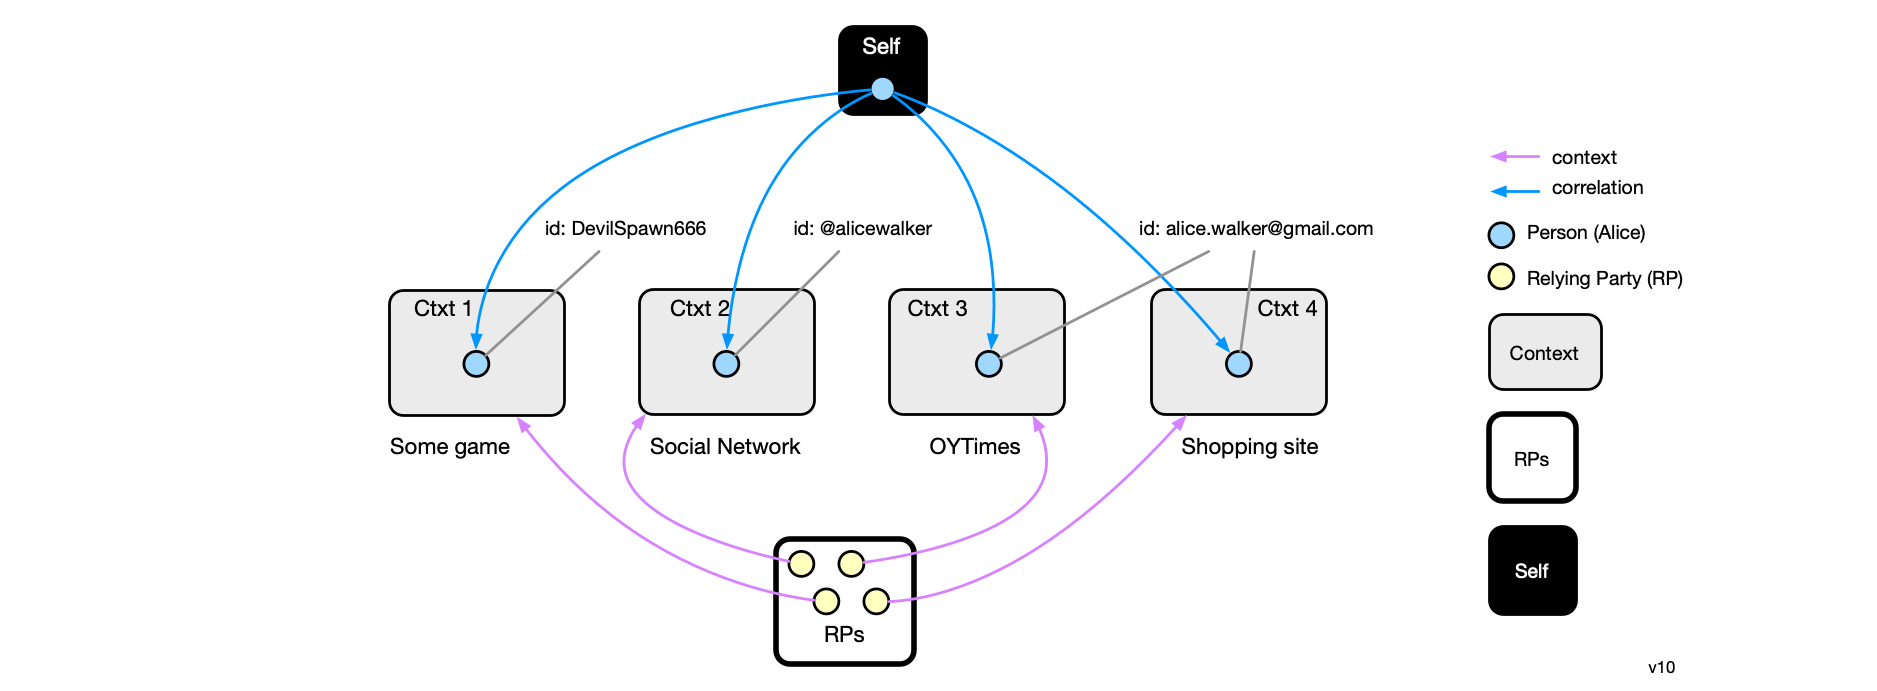
\includegraphics[width=\textwidth]{./images/example2.png}
\caption{Alice's Self and Relying Parties}
\label{fig:RPs-container}
\end{figure}

The personal information flowing through the connections may flow from the identity agent, to the identity agent, or in both directions. It may have originated on either side. It may be self-asserted claims (attributes) entered by the person directly into the identity agent, or it may be claims entered by the person using an app, or sensed by a local app's sensor, or generated by the other party based on direct on-site or on-app interactions with the person.

\subsubsection{Container classes}

We describe the data model in two parts. The first part describes the data containers. The second describes the data held by these containers. Let us start describing the data model of the containers themselves. Figure~\ref{fig:containers} shows the various data container classes. 

\begin{figure}[h!]
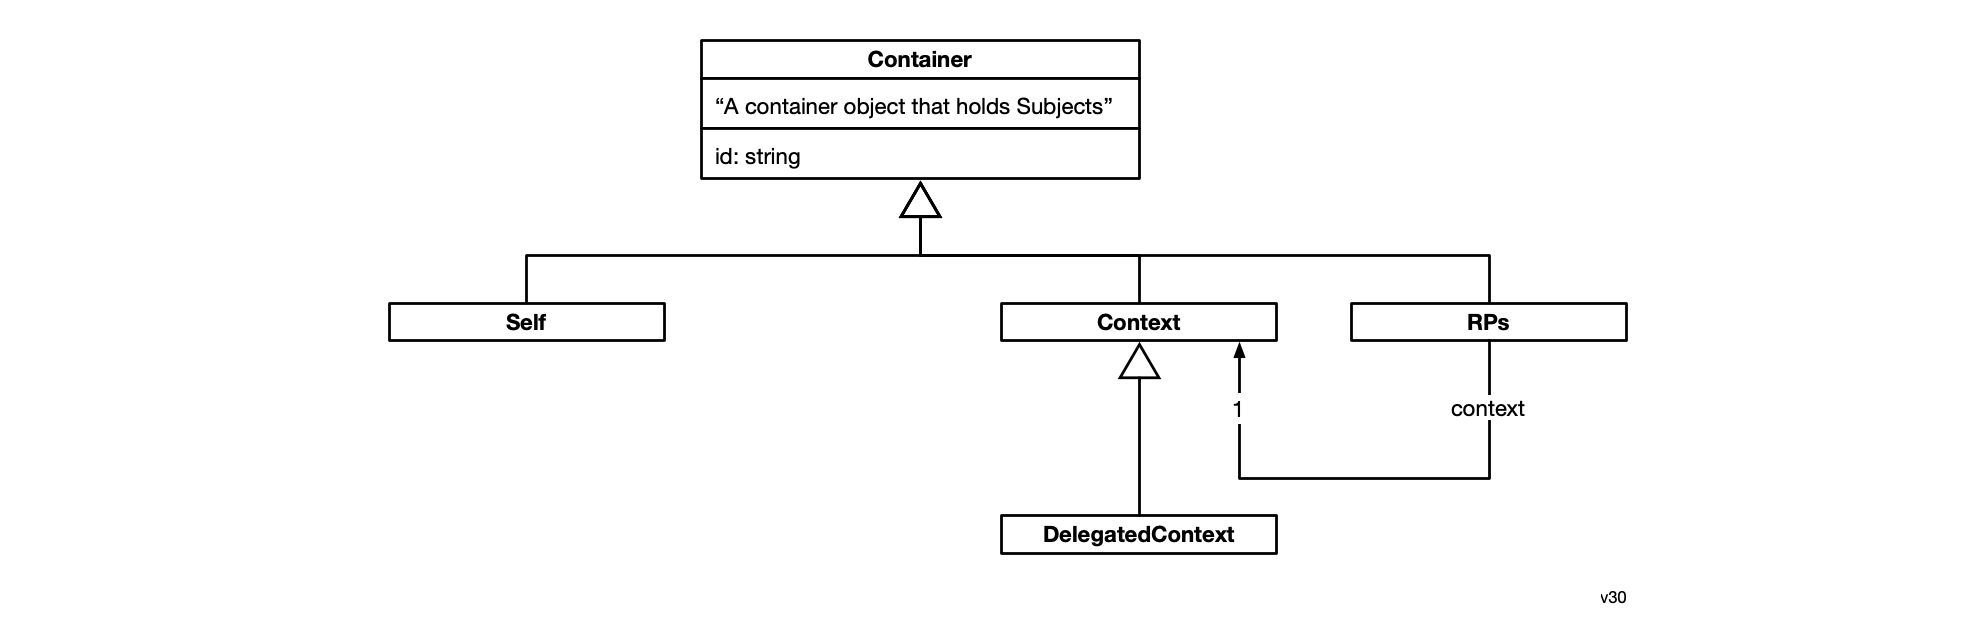
\includegraphics[width=\textwidth]{./images/container-classes.png}
\caption{Container classes}
\label{fig:containers}
\end{figure} 

\textbf{Classes}

\begin{itemize}
	\item \textbf{RPs} - a container holding a set of Relying Party (RP) nodes (see Identity Agent Classes). Each RP node represents a party with which the person has a connection. These RPs may be other people or corporations, such as a digital service provider. Each RP has the following properties:
	\begin{itemize}
		\item \textbf{Context} - a single Context that captures one aspect of the connection between the user and some RP.
	\end{itemize}
	\item \textbf{Self} - the single data Container holding a single Person node that represents the selfness of the user.
	\begin{itemize}
		\item \textbf{id} - user identifier (e.g. email)
	\end{itemize}
	\item \textbf{Context} - a Container holding a Person node that represents the user in a specific aspect of their relationship (called a \emph{Connection}) with some RP. 
\end{itemize}

\textbf{More about Contexts}

A Context is a Container holding a Person node that represents the identity agent user in a specific aspect of their relationship (called a \emph{Connection}) with some RP. We say ``specific aspect'' because the relationship between the person a given other, may be represented by more than one context, each representing a different aspect. A Context has the following attribute:

\begin{itemize}
\item \textbf{protocols[]} - array of one or more Protocol instances.
\end{itemize}

The kinds of data held by a context depends on the communications protocol (using the term loosely) between the agent and the other party. 

The \emph{DelegatedContext} subclass of Context is described in its own section below.

\textbf{Protocols}

A Protocol class represents a communications protocol used between the identity agent and an endpoint provided by another party. Each subclass represents a different communications protocol such as SIOPv2, GoogleAccountSync, BasicMessage (DIDComm), etc.  

A Context has one or more Protocols. Figure~\ref{fig:protocol} shows an example of Alice who has a connection with LinkedIn. This connection's Context that contains the information that Alice shares with the LinkedIn via the OpenID Connect SIOPv2 protocol. Note: this example is hypothetical, since LinkedIn does not currently support SIOPv2.

\begin{figure}[htbp]
	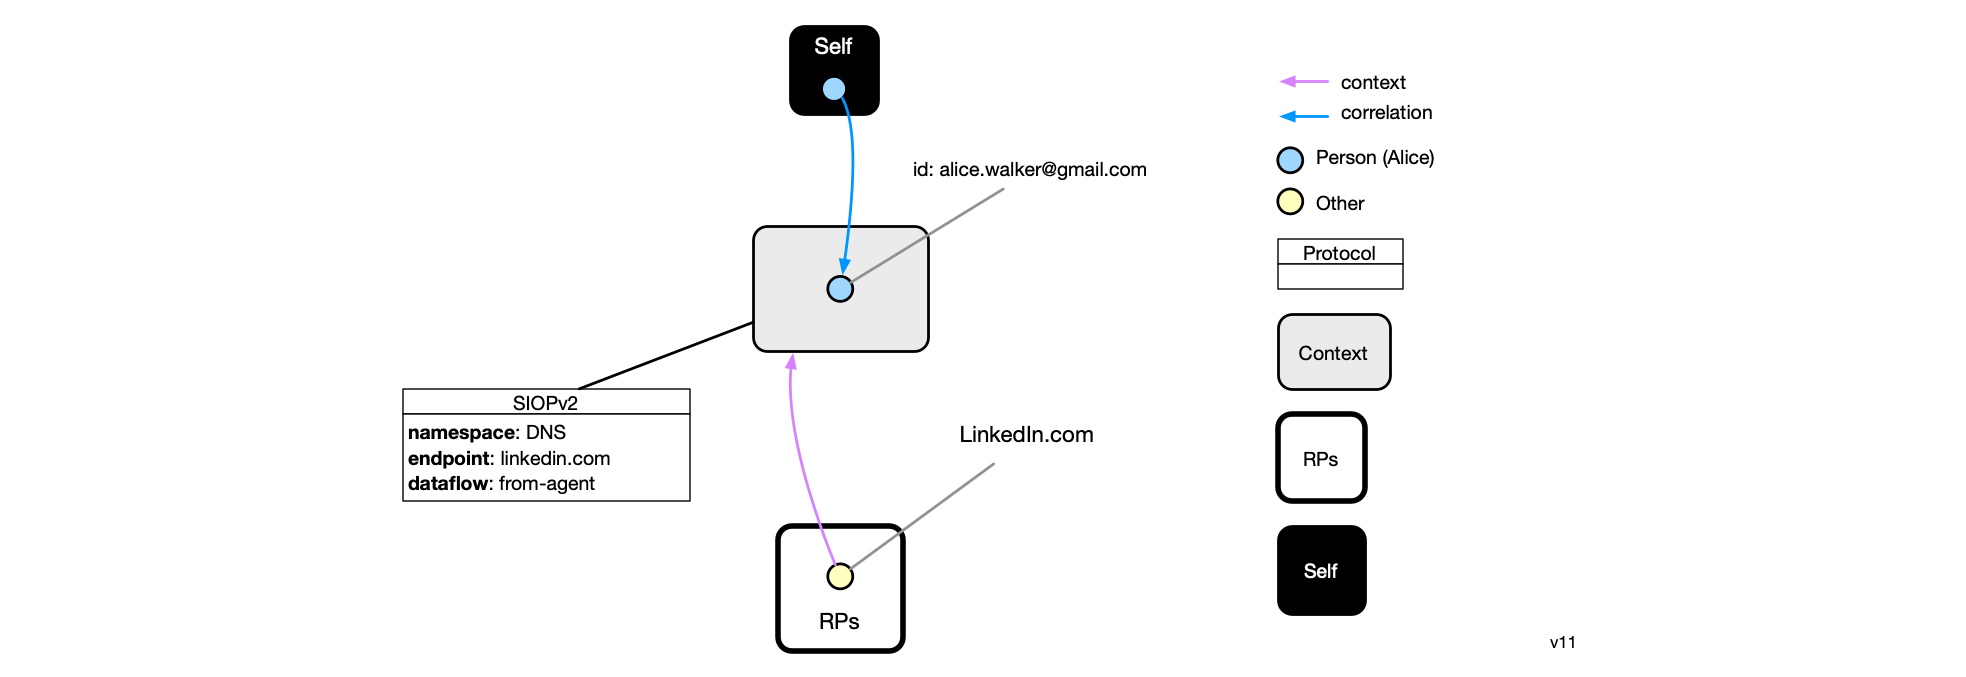
\includegraphics[width=\textwidth]{./images/context-with-protocol.png}
	\caption{Protocols}
	\label{fig:protocol}
\end{figure}

Figure~\ref{fig:n-protocols} extends the previous example by showing the use of multiple Protocols. In addition to the hypothetical SIOPv2 protocol, the connection depicted also leverages a web scraping/filling Protocol to capture her data from the LinkedIn website. Lastly, the connection's context also uses the Mee Data Network protocol to allow the context's data to be exchanged with other apps and agents on this  network. 

\begin{figure}[htbp]
	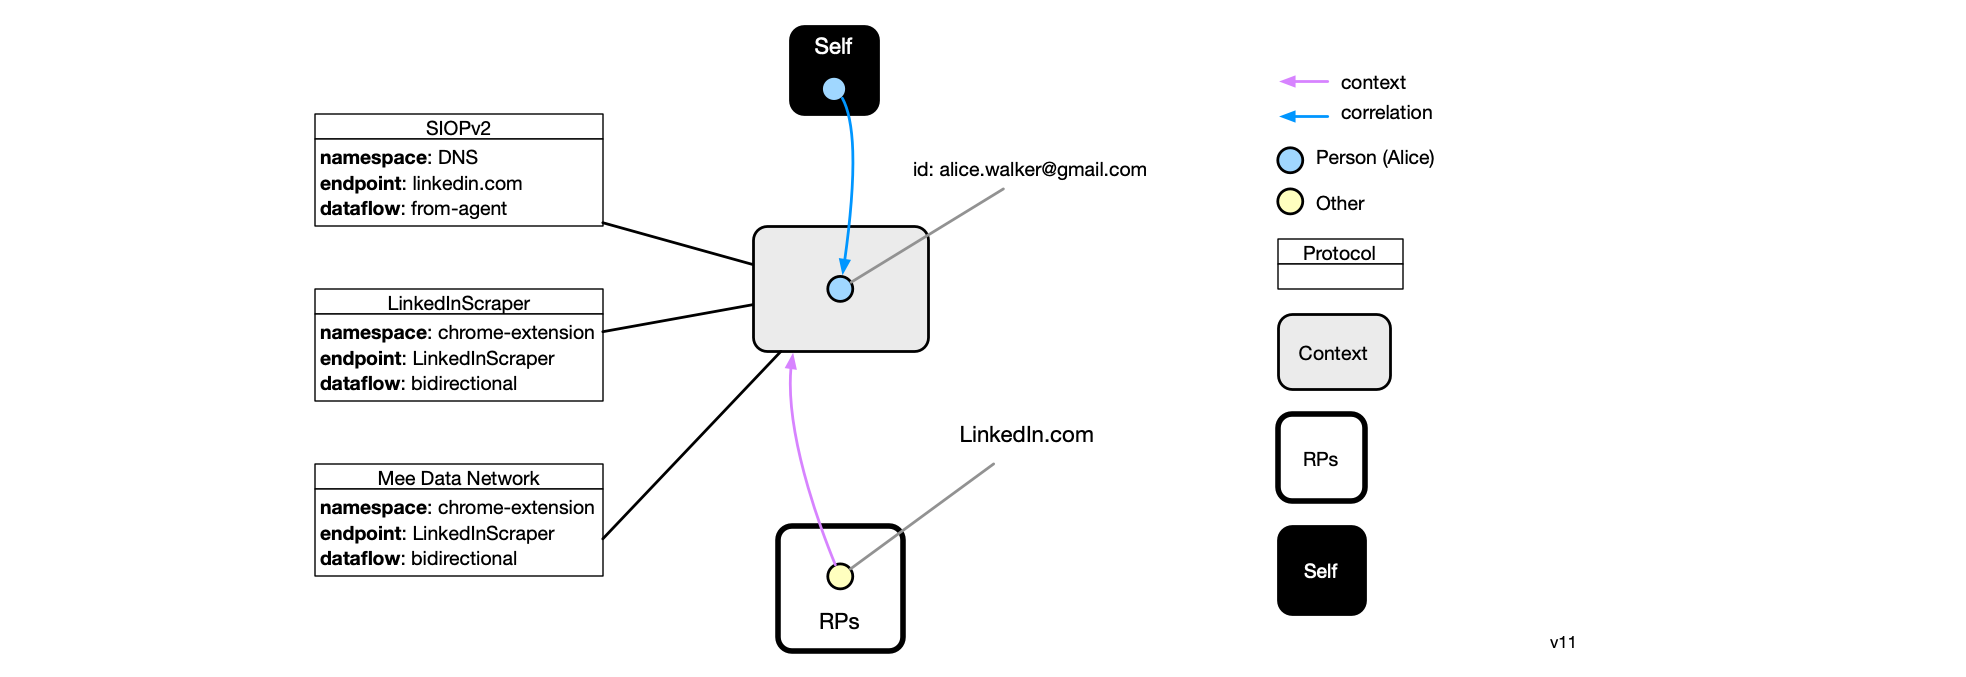
\includegraphics[width=\textwidth]{./images/context-with-n-protocols.png}
	\caption{Context with multiple protocols}
	\label{fig:n-protocols}
\end{figure}

Each Protocol instance has these attributes:
\begin{itemize}
\item \textbf{namespace} - a string that indicates the namespace used by the ``endpoint'' attribute
\item \textbf{endpoint} - a string identifier that unique identifies the other party with which the person has a relationship within the above namespace attribute
\item \textbf{dataflow} - one of {to-identity agent, from-identity agent, bidirectional} - indicates the direction of data flow between the identity agent and the endpoint
\end{itemize}

\textbf{Multiple connections}

In the example shown in Figure~\ref{fig:groups}, we expand our story about Alice. Alice has five connections contextualizing her relationships with each of five organizations and/or people. We discuss each connection moving left to right in the diagram:

\begin{itemize}
	\item \textbf{Bob}. Alice has a connection to Bob. It has a   context and uses the DIDComm BasicMessage protocol (which uses a DID identifier).
	\item \textbf{Some game}. Alice has a connection with a game she likes to play. It contains a context representing this game. She uses id ``DevilSpawn666'' as her identifier in this context.  
	\item \textbf{X}. Alice has a connection to X social network. It contains a context representing her X account. Her id is ``@alicewalker'' on X.
	\item \textbf{Google Account}. Alice has a connection to her Google account. It consists of a context that contains the attributes of her Google account. This context uses her ``awalker@gmail.com'' id. 
	\item \textbf{Olde York Times}. Alice has a connection to the Olde Yorke Times (hypothetical) news media site using four protocols. The context captures her sign-on relationship using OpenID SIOPv2 protocol using her id ``0x3443f23135839''. The context holds information she has entered using a form filler as well as her account information managed by this site. 
\end{itemize}

\begin{figure}[htbp]
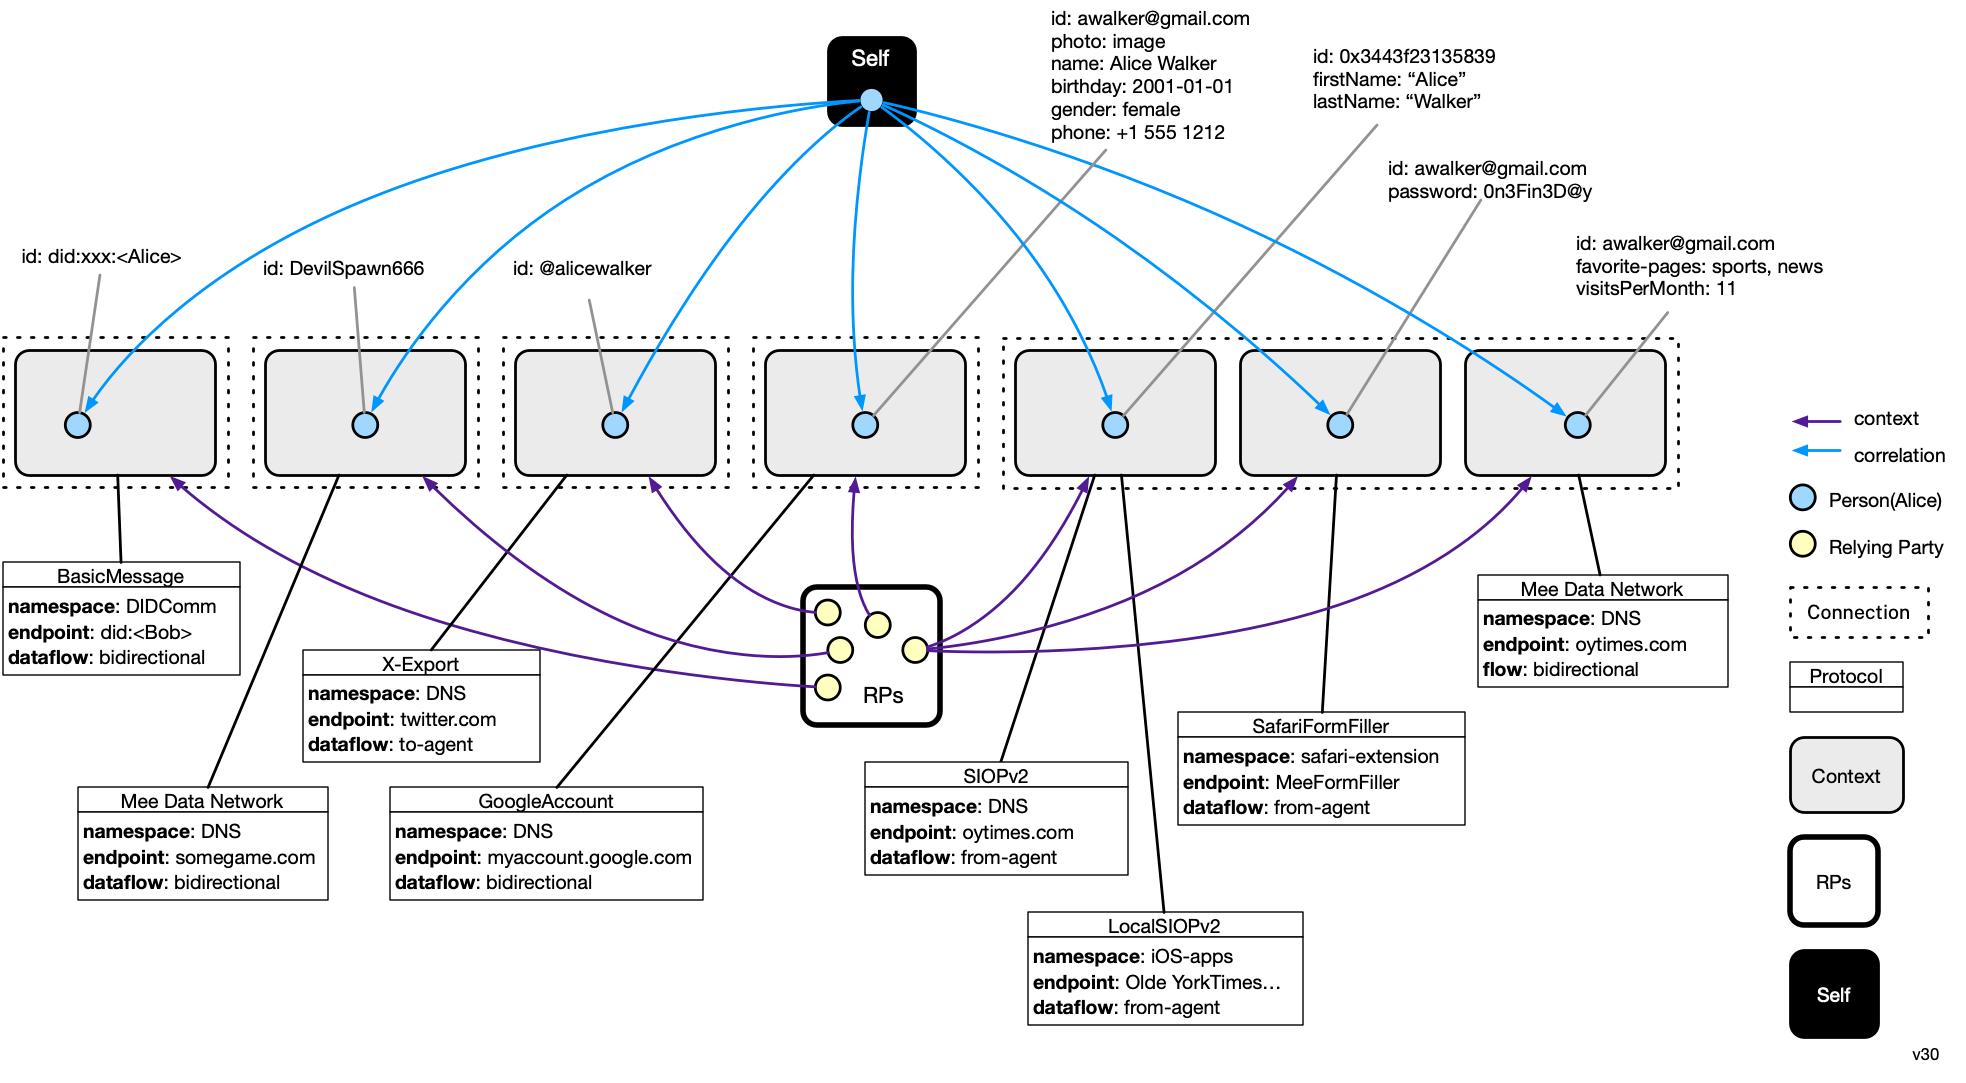
\includegraphics[width=\textwidth]{./images/multiple-connections.png}
\caption{Alice's five connections}
\label{fig:groups}
\end{figure}

A relationship between the agent and another party is called a \emph{connection}. It is represented by one or more other contexts each of which has a protocol (and sometimes more than one). Alice is shown with five connections--one for each of the five RP nodes in her RPs container. 

\textbf{Delegated Contexts}

Alice takes care of her elderly mother, and helps her mother manage her bank account at Santander Bank. Her mother has an agent containing a connection to her bank, the data for which (e.g. her mother's OpenID Connect SIOP claims) is stored in one of the contexts representing this connection. Using her identity agent, Alice's mother has delegated access to this context to her daughter Alice.

\begin{figure}[htbp]
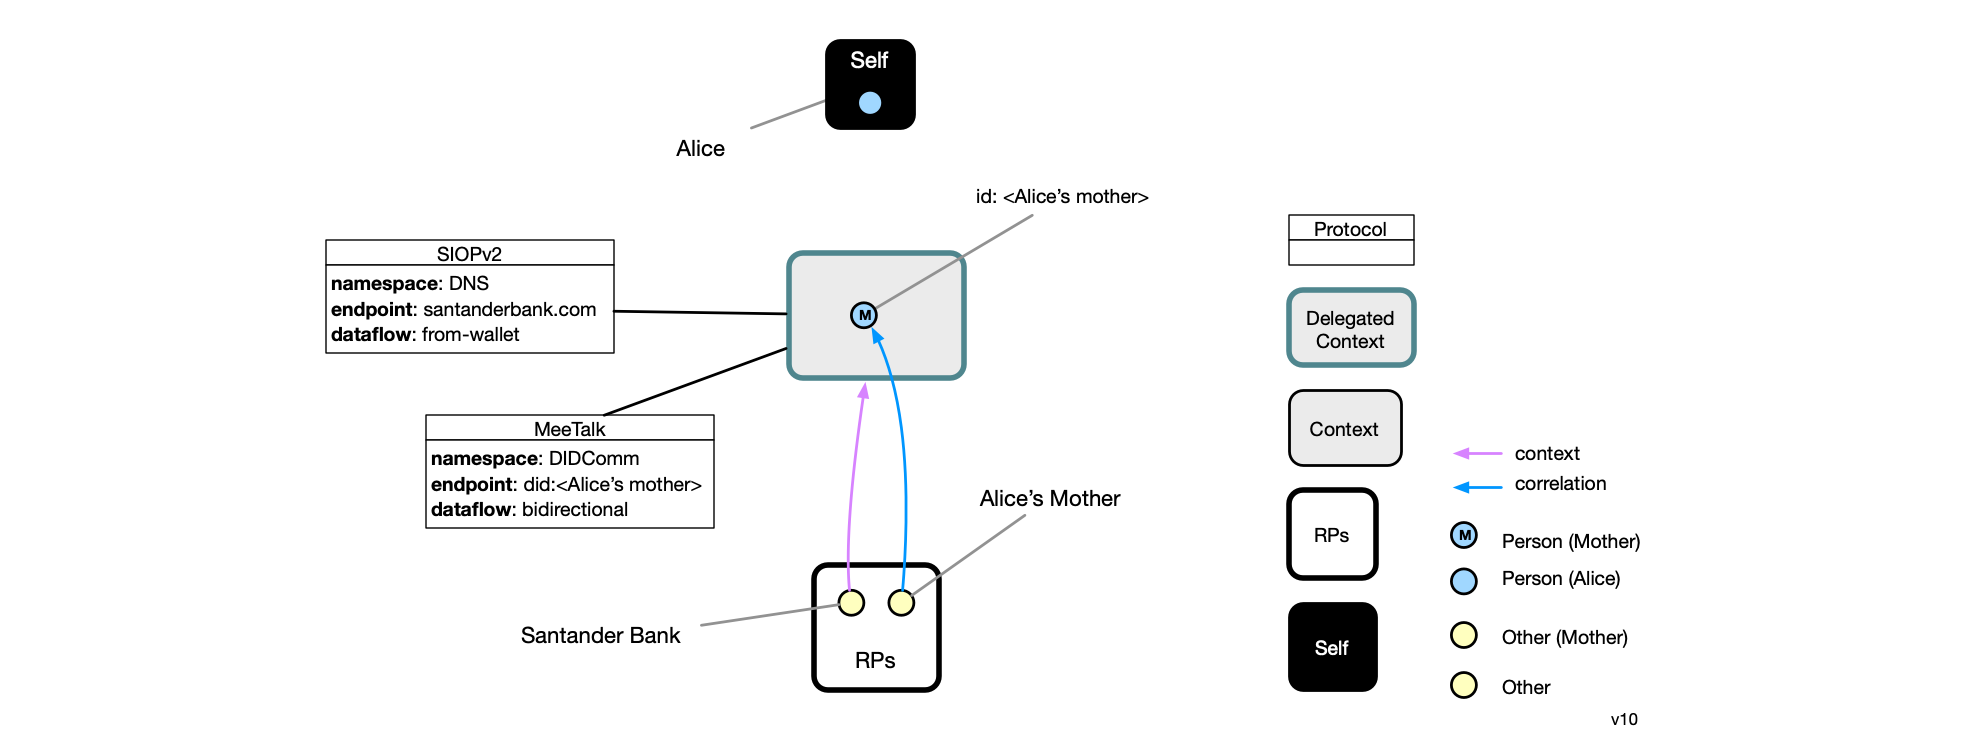
\includegraphics[width=\textwidth]{./images/delegated-contexts.png}
\caption{Alice's identity agent with a connection using a delegated context}
\label{fig:delegated-contexts}
\end{figure}

As shown in Figure~\ref{fig:delegated-contexts}, Alice's mother's connection with her bank is represented by a delegated context. Alice now has the ability to view (and potentially update) information in this context. Information about her mother's account information at the bank might be helpful for Alice to have while taking care of her mother. Data replication/synchronization is used to ensure that Alice's DelegatedContext is always synchronized with the ``original'' context on her mother's identity agent.

\subsubsection{Identity Agent Classes}

Group and context containers contain information about subjects (things) that are described according to the \emph{Persona} schema. In knowledge representation parlance, the Persona schema would be known as an \emph{upper ontology}.

In the Persona schema, people are represented as instances of Person, a \emph{PersonalAccount} class is also defined. These classes are shown below. 

\begin{figure}[htbp]
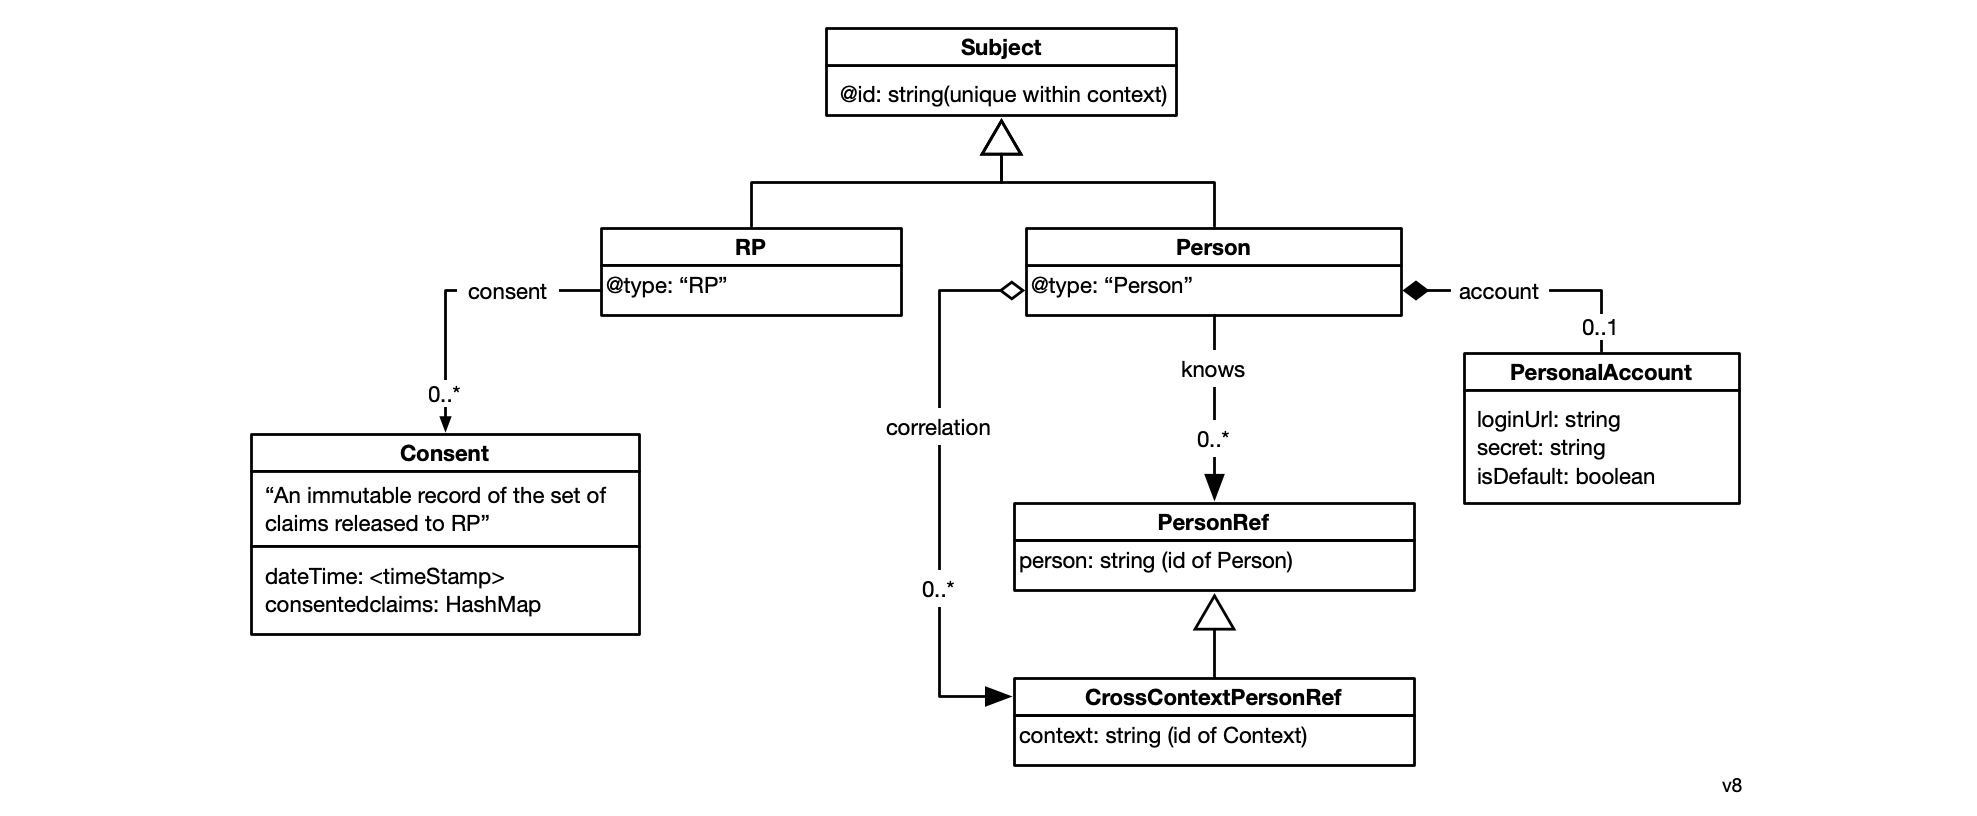
\includegraphics[width=\textwidth]{./images/persona-classes.png}
\caption{Persona schema}
\end{figure}

\textbf{Classes}

\begin{itemize}
\item \textbf{Subject} - kind of digital subject about which the identity agent stores information
\item \textbf{Person} - a natural person, a subclass of Subject. Each person has the following properties:
	\begin{itemize}
	\item \textbf{claims[]} - a set of zero or more properties. These properties may be structured (e.g. a physical address (e.g. from vCard)) or scalars. Here are a few examples of scalar \emph{claim} properties: 
		\begin{itemize}
		\item givenName
		\item familyName
		\item phoneticGivenName
		\end{itemize}
	\item \textbf{account} - an optional PersonalAccount at some other party's site or app
	\item \textbf{correlation} - zero or more CrossContextPersonRefs each of which acts as a link to a target Person object in another Context. Both the source Person and the target Person can be thought of as contextualizations of the same underlying person.
	\item \textbf{knows} - zero or more PersonRefs that link to a Person representing some other person (other than the  agent user) in the same context
	\end{itemize}
\item \textbf{RP} - a Subject representing another person or a legal entity with which the identity agent user has a connection. Each RP object has:
	\begin {itemize}
	\item \textbf{consents} - zero or more Consent objects. Each Consent has:
		\begin{itemize}
		\item \textbf{dateTime} - time stamp of when the user consented to share this set of claims
		\item \textbf{claims[]}  - a set of zero or more claims (note: claim types (e.g. ``email address") not their values)
		\end{itemize}
	\end{itemize}
\end{itemize}

\textbf{Extensions}

Each protocol class will extend the Persona schema by defining Person subclasses, other new object classes and new kinds of relationships. For example the \hyperfootnote[Google Account][https://]{myaccount.google.com}  API includes (optional) claims of ``name", ``gender" and ``birthday". The protocol that supports the myaccount API would define these claim types in its schema, and insert a link to this schema in its corresponding context's \emph{schema} attribute.

\subsubsection{Datatypes}

This section is largely incomplete, but will eventually describe lower level classes that we call \emph{datatypes} that are used by the higher level classes mentioned above. Some datatype classes are shown in Figure~\ref{fig:datatypes}.

\begin{figure}[htbp]

\includegraphics[width=\textwidth]{./images/datatypes.png}
\caption{Datatypes}
\label{fig:datatypes}
\end{figure}

\begin{itemize}
\item \textbf{EndpointId} -  an identifier of an endpoint (e.g. web service or a local app) supported by another party.
\item \textbf{LocalAppId} - an EndpointId that identifies a service provider's mobile application. 
\item \textbf{URL} - an EndpointId that identifies a service providers's web service using a traditional URL
\item \textbf{DID} - an EndpointId that identifies a service using a \hyperfootnote[DID][https://]{www.w3.org/TR/did-core/}
\end{itemize}

\begin{comment}{\textbf{Secret Recovery Phrase} - a 12-word textual phrase that the person creates. It is used to generate cryptographic keys that in turn are used to encrypt the person personal data whether it is stored locally on their device or in a backup location. It can be used to generate keys to digitally sign transactions (e.g., for crypto currency transactions). It should never be shared with anyone or any service provider. If the person loses this phrase, they lose the ability to decrypt their data. 
}
\end{comment}

\section{Mee Data Network} % SECTION 

Although agents can form connections with many kinds of existing apps using a variety of protocols, we describe here a network of apps and agents called the Mee Data Network that use a specific set of protocols and adhere to a specific trust framework. These two, taken together, offer agent users particularly strong privacy guarantees.

\subsection{Private data sharing and the Mee Data Network}

It is obvious that data held and/or managed by a user's agent and stored locally on a device the user owns, is inherently under this user's control. The challenge is that data that a user shares with another party or that is collected by that party in other ways \emph{also} needs to be under the user's control. Unfortunately, it is impossible using solely technical means to remotely control data held by another party. Privacy laws and regulations on the other hand, while intended to provide this control, in practice place such burdens on the user to effectuate this control that it hardly exists. The solution is to combine both legal (license agreements) and technical means (identity agents and apps on the Mee Data Network). 

The legal mechanism we propose is the \hyperfootnote[Mee Data Network License (MDNL)][https://]{docs.google.com/document/d/13aGk5adoncMxxfl5637NfqP6fl6q\_op\_1CF50UrJNjg}. The MDNL is a pairwise contract between two parties. The first is the service provider providing an app. The second is an organization that represents the community of identity agent users (e.g. The Mee Foundation). This organization acts as a \emph{Mediator of Individual Data} (MID), a term coined by Lanier et al.\cite{Lanier2018}, that enforces the terms of the MDNL on behalf of the community. 

The MNDL imposes obligations on the app provider, among which is the requirement to respect the user's \emph{data rights} to access, correction (editing), and deletion of the information collected and held by them. The MNDL covers information that the user may have shared manually (e.g. by filling in a form, or other kinds of on-app interactions) or shared with them by a person's identity agent. The MNDL requires the provider to implement \emph{data rights} APIs that an identity agent uses to remotely control this app-held data. In this way, we tie the legal (MDNL) and technical means (identity agents and APIs) together.

The MDNL's provisions are intentionally generic. They are designed to meet the needs of the entire community of identity agent users. We expect that other contracts containing more specific provisions will be required to meet the needs of more specialized communities. Each community can amend the MDNL to meet the specifics they require, provided that they do not weaken the MDNL's existing provisions and protections. These specialized communities would organize, govern and operate independent MIDs that enforce their more specialized MDNL-based contracts. These specialized MIDs would enter into agreements with one or more providers which would be held to both the generic terms of the MDNL and the additional, specialized terms.

\section{Acknowledgements}
Contributors to this paper include Kirill Khalitov, Alexander Yuhimenko, Sergey Kucherenko, Maria Vasuytenko, Vlad Fisher, and Xenya Shatalova.

\bibliography{../library}
\bibliographystyle{plainurl}

\end{document}  